\chapter{Sistema propuesto (teoría y simulaciones)}

Se propone un sistema de comunicaciones óptico con una estructura de hub como se aprecia en la figura \ref{fig_hub}. Utilizando este Diseño físico con una etapa adicional de codificación y correccion de errores. El hub central es una etapa totalmente óptica que puede o no estar amplificada. Con la amplificacion optica se incrementa notablemente el rango, de 5 km a mas de 20 km.
La pila de codificación se detalla en la figura \ref{fig_stack} donde puede verse un arreglo convencional, excepto en la ultima 

\begin{figure}[t]
\centering
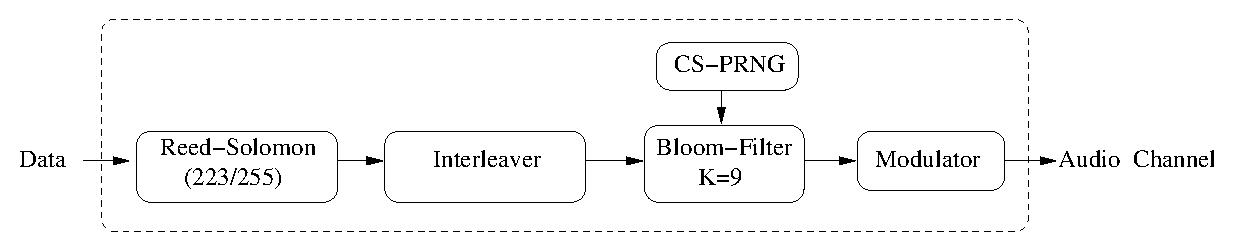
\includegraphics[width=0.9 \textwidth]{Soft-stack2.eps} 
\caption{Etapas del sistema de comunicaciones}
\label{fig_comstack}
\end{figure}

\section{Códigos correctores de errores}

Todo sistema de comunicaciones posee errores que deben ser corregidos antes que los datos sean procesados. Una técnica muy utilizada es la de utilizar un algoritmo de detección y retransmisión.
La idea de un código corrector de errores esta relacionada con la técnica de espectro expandido, siendo ambas métodos que ayudan a la transmisión de la información reduciendo la entropía de la información transmitida, o lo que es lo mismo, aumentando la redundancia de la información. En particular, los sistemas de comunicaciones modernos hacen uso de los métodos de Forward Error Correction (FEC) que no necesitan de retransmisiones.



\subsection{Reed-Solomon}
Se utilizó un codigo de Reed-Solomon standard 223/255, esto significa que se tienen 32 bytes de paridad por cada 223 bytes de datos, y se pueden corregir hasta 16 bytes. Se utilizo la librería de Phil Karn, y no se utilizaron los bits de sindrome para mejorar la correccion. Todo error conocido es descartado.
Con posibilidad de error de simbolo P, la posibilidad de error de un codigo reed-solomon R(n/k) es:
$$P_{rs}= \sum_{k=(\frac{n-k}{2}+1)}^{n} \binom{L}{i} * P^{i} * (1-P)^{L-i} $$

\subsection{LDPC}
El esquema de corrección de errores LDPC (Low Density Parity Check) es muy utilizado actualmente debido a su gran capacidad de corrección de errores, en algunos casos muy cercana a la máxima capacidad teórica del canal.
Antes de ahondar en la descripción de este algoritmo cabe aclarar que a pesar de ser utilizado para ciertos modelos durante la primera fase de la investigación, fue descartado en la versión final por un modelo mas simple y con menos requerimientos de hardware que presenta una performance similar desde el punto de vista de corrección de errores.
Básicamente es un código lineal que utiliza una matriz de paridad grande y dispersa.
La matriz H es tal que cualquier codeword valido x cumple con $H*x=0$

\paragraph{LDPC: Generador de matriz}
La matriz generadora puede crearse facilmente si H es de la forma $[D|I]$, simplemente formando la matriz:
$$G=[I|D']$$
Donde D' es la transpuesta de la matriz D
Para la generacion de la matriz se opto por utilizar un algoritmo random y luego aplicando algunos tests, para lograr una matriz sistemática de rate entero (1/2, 1/3, etc.)
Para verificar se G genera vectores cuya matriz de paridad es H, puede verificarse que:
$$ H*G'=0 $$

Podemos definir la matriz de paridad H como una matriz de paridad que tenga mas de 3 unos por fila y una cantidad similar por columna. Buenos resultados se obtienen a partir de matrices de 200x100.
Se puede comenzar por una matriz vacía $H = 0$ del tamaño deseado, y ir agregándole unos al azar. Cierto análisis es necesario para garantizar que no se cumplan ciclos y que la cantidad de unos por columna y por fila es la deseada. De esto se encargan los algoritmos llamados evencol y evenrow.

El generador puede generar matrices de cualquier tamaño, de esta manera:

$$ ./genMatrix <width> <height> <ones per row>$$

La matriz se genera en la salida estandard. El formato es el utilizado por la libreria boost:ublas.

NOTA: La matriz siempre esta compuesta de simbolos en GF(2) (O sea, ceros y unos)

\paragraph{LDPC: encoder}

El vector inicial se toma de la entrada estandard y el codeword se emite en la salida estandard. La sintaxis es muy sencilla:

$$ ./ldpcen <matriz> < in >out $$
\paragraph{LDPC: decoder}
Si se invoca este filtro mediante el nombre decodificador, tomara el codeword de la entrada estandard, aplicara el algoritmo de belief-propagation (Hard-decision) y se emite el vector original por la salida estandard:
La diferencia radica que en nuestro caso, al ser un canal asimetrico no se permite el bit-flip de un valor cero a un valor uno, ya que es imposible que se produzca ese error.
La linea de comando es la siguiente:

$$ ./ldpcdec <matriz> <in >out $$

La conversion codeword->vector es sencilla, ya que al ser un codigo sistemático solo se necesita eliminar la parte del vector que representa la paridad añadida.

Se generaron muchas matrices, desde 256x128 hasta matrices muy grandes de 10000x5000, pero el tiempo de decodificacion crece enormemente para matrices grandes.

\paragraph{LDPC: optimizacion}

Debido a la naturaleza iterativa del decodificador ldpc, pronto se convirtio en el cuello de botella de la simulacion. Para acelerar el sistema, se opto por realizar la siguiente optimizacion:
LDPC consta basicamente de varios loops, dentro de los cuales se accede a la matriz de paridad, y a otras matrices que acumulan datos intermedios. Primeramente la implementacion fue realizada como mencionamos utilizando boost:ublas, pero luego se comprobo que una implementacion utilizando arrays de C era hasta 3 veces mas rapida.
Luego se procedio a realizar un algoritmo de ``unrolling'' de estos loops, generando codigo especifico a una matriz dada, sin ningun tipo de loop. Obviamente este codigo es mucho mas grande, pero la aceleracion provista es aun mayor, del orden de 8 veces mas rapido que en implementaciones iniciales.
La manera de invocar el generador de codigo es la siguiente:

$$ ./genLdpcDecoder matriz  > decodeGen.h $$

El archivo generado decodeGen.h es el decodificador especifico para la matriz dada. Este header de C es luego incluido desde el decodificador ldpcenc.cpp y compilado. Al ser generalmente un archivo de un megabyte para una matriz pequeña de 1024x512, el proceso de compilacion el largo y requiere de mucha memoria.
Por otra parte, no se optimizo el proceso de codificacion ldpc, ya que consiste solo de una multiplicacion de un vector por una matriz, y es una de las tareas en la que boost:ublas es especialmente eficiente.

\section{Canal Z con filtros de bloom}

En esta sección vamos a modelar el canal por el cual estamos transmitiendo datos, específicamente el modelo de ruido del mismo. Es este modelo de ruido, distinto de canales convencionales como por ejemplo ruido Gaussiano, que nos permite innovar en el diseño de algoritmos.
Empezaremos primeramente estudiando un modelo simplificado del canal por el cual vamos a trasmitir, un simple canal simétrico binario, para despues ahondar en un caso especial de este mismo, denominado Canal Z.
\begin{figure}[t]
  \begin{center}
    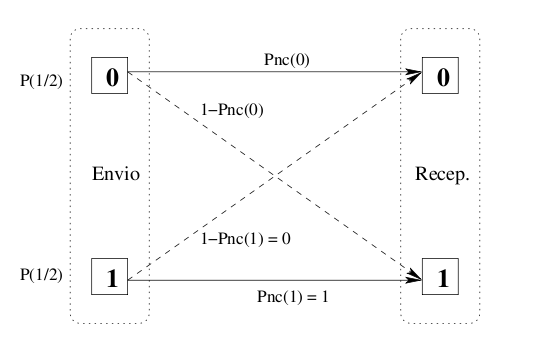
\includegraphics[scale=0.43]{capacidad/canalBinario.png}
  \end{center}
\caption {Canal binario: esquema de probabilidad}
\label{fig:canbin}
\end{figure}

Para calcular el ruido en un canal simétrico binario, calculamos la probabilidad de no-colision que tendra un usuario determinado, ya que las colisiones seran el ruido del canal (En esta etapa no consideramos otros tipos de ruido que pueda tener el canal físico).

\noindent Cantidad de slots por trama: $m$
\noindent Cantidad de usuarios: $n$

\noindent Probabilidad de no colisión para un usuario en un canal simétrico:
\begin{equation}
P_{nc}=\left(\frac{m-1}{m}\right)^{n-1}
\end{equation}


\noindent Probabilidad de no colisión para un usuario en un canal óptico:
\begin{eqnarray}
P_{nc} & = & P(1) \cdot P_{nc}(1) + P(0) \cdot P_{nc}(0) \\
P_{nc} & = & \frac{1}{2} \cdot 1 +  \frac{1}{2} \cdot \sum_{i=0}^{n-1} 
C^{n-1}_{i} \left(\frac{m-1}{m}\right)^i  \left(\frac{1}{m}\right)^{n-1-i}  \left(\frac{1}{2}\right)^{n-1-i} 
\end{eqnarray}

\noindent Donde $\left(\frac{m-1}{m}\right)^i$ es la probabilidad de no
colisión de $i$ canales (se suma para todo posible número de canales no
colisionando: $1\leq i\leq n$, que están en otro slot), $
\left(\frac{1}{m}\right)^{n-1-i}$ es la probilidad de colisión de los restantes
$n-1-i$ (estos están en el mismo slot que el canal actual, el `$-1$' es para no
contar el canal actual), y la colisión se produce cuando los otros canales
transmiten $1$ cuya probabilidad es $\left(\frac{1}{2}\right)^{n-1-i}$. El
factor $C^{n-1}_{i}$ suma sobre todas las combinaciones posibles de canales no
colisionando, que son hechos independientes.

\noindent Teniendo en cuenta que $ \sum_{i=0}^{n-1}
C^{n-1}_{i} \left(\frac{m-1}{m}\right)^i  \left(\frac{1}{2m}\right)^{n-1-i}$ es la potencia $n-1$ de un binomio, reemplanzando tenemos
\begin{eqnarray}
P_{nc} & = & \frac{1}{2} +  \frac{1}{2} \cdot \left(\frac{m-1}{m} + \frac{1}{2m} \right)^{n-1} \\
P_{nc} & = & \frac{1}{2} +  \frac{1}{2} \cdot \left(1- \frac{1}{2m} \right)^{n-1} \\
P_{nc} & \simeq & \frac{1}{2} +  \frac{1}{2} \cdot e^{-1/2} 
\end{eqnarray}

\noindent Donde la última aproximación vale para $n=m$ y $n$ grande.


\vspace{5mm}

\noindent Para el caso de {\em bloom} filters con $k$ filtros\footnote{Se envían $k$ repeticiones del bit en canales distintos, entonces basta que sólo uno de ellos sea 0 para que recibamos un 0 en un canal óptico.} la probabilidad de no colisión es:
\begin{eqnarray} 
P_{nc}^{k} & = &  P(1) \cdot P_{nc}^{k}(1) + P(0) \cdot P_{nc}^{k}(0)\\ \label{Pnc_k}
\end{eqnarray}
Sabiendo que la probabilidad de no colisión para el 0 es:
\begin{eqnarray}
P_{nc}^{k}(0) & = & 1 - \big(P_{c^k}(0)\big)^k 
\end{eqnarray}
Pero la probabilidad de colisión para el 0 cuando se transmiten $k$ copias es:
\begin{eqnarray}
P_{c^k}(0) & = & 1 - \big(P_{nc^k}(0)\big)  \enspace,
\end{eqnarray}
y que además la probabilidad de no colisión para los $k$ slots del bloom
filter es
\begin{eqnarray}
P(\mbox{no col.} k) &=& P(\mbox{no col.}1)\cdot P(\mbox{no col.}2)\cdot P(\mbox{no col.}3)\cdots P(\mbox{no col.}k)\\
&=&\left(\frac{m-1}{m}\right)\cdot\left(\frac{m-2}{m-1}\right)\cdot\left(\frac{m-3}{m-2}\right)\cdots\left(\frac{m-k}{m-(k-1)}\right)\\
&=& \frac{m-k}{m} \enspace.
\end{eqnarray}
Luego la probabilidad de colisión con alguno de las $k$ copias del bit es
\begin{eqnarray}
P(\mbox{col.}k)&=& 1-P(\mbox{no col.} k)\\
&=& 1-\frac{m-k}{m}\\
&=& \frac{k}{m} \enspace.
\end{eqnarray}
Entonces reemplazamos y calculamos:
\begin{eqnarray}
P_{c^k}(0) & = & 1 - \left(\sum_{i=0}^{n-1} C^{n-1}_{i} \left(\frac{m-k}{m}\right)^i \left(\frac{k}{2m}\right)^{n-1-i} \right)  \\
& = &  1-\left( 1-\frac{k}{2m}\right)^{n-1}
\end{eqnarray}
Reemplazando esta ecuación en~\ref{Pnc_k} obtenemos:
\begin{eqnarray}
P_{nc}^k & = & \frac{1}{2} + \frac{1}{2} \left( 1- \left( 1- \left( 1- \frac{k}{2m} \right)^{n-1}  \right)^{k}  \right) 
\end{eqnarray}

Sin embargo, este calculo es incorrecto, comparandolo con los datos que da el simulador. La formula entrega valores de error menores con respecto a los reales, como se observa en la figura. 
Los trazos del mismo color corresponden a el mismo K con azul(K=1), verde (K=2) y rojo(K=4). M=256

\subsection{Entropía}

Comenzemos por lo básico:

Segun Shannon, el \textbf{contenido de informacion} h(x) de un suceso x dada la posibilidad que suceda P(x) es:
$$ h(x) = log_{2}\left(\frac{1}{P(x)}\right) $$

Y la entropia de un conjunto A, H(A) se define simplemente como el promedio del contenido de información:

$$ H(A) = \sum_{x E A_{x}} P(x)log_{2}\left(\frac{1}{P(x)}\right)$$

En un canal binario solo dos sucesos existen, uno con probabilidad p, y otro con probabilidad 1-p, por lo tanto para p siendo la probabilidad de error:

$$ H(p) = -p log_{2}(p)-(1-p)log_{2}(1-p) $$

\subsection{Entropia condicional}

Vamos a analizar la entropia de dos conjuntos X de entrada y Y de salida interrelacionados.

La entropia condicional de X dado $y=b_k$ donde $b_k$ es un valor dado, es la entropia de la distribucion de probabilidad $P(x|y=b_{k})$:
$$H(X|y=b_{k}) = \sum_{x \in A_{x}} P(x | y=b_{k})\log_2\left(\frac{1}{P(x | y=b_{k})}\right) $$

La entropia codicional de X dado Y es el promedio, sobre y, de la entropia condicional de X dado y:
$$H(X|Y) =  \sum_{xy \in A_{x}A_{y}} P(x,y)\log_2\left(\frac{1}{P(x,y)}\right) $$

\subsection{Información mútua}
La información mútua entre X e Y es:
$$I(X;Y) = H(X)-H(X|Y)$$
Mide el promedio de reduccion de la incertidumbre acerca de x que resulta de saber el valor de y, o viceversa: la cantidad promedio de informacion que x revela acerca de y.

\subsection{Capacidad de canal}

La capacidad C de un canal discreto sin memoria es :

\begin{equation}
C = \max_{{\cal{P}}_x} I(X;Y) 
\end{equation}

O sea, la máxima información mutua entre los alfabetos X de entrada e Y de salida.
Para hallar el maximo podemos derivar $I(X;Y)$ con respecto a la probabilidad $P_x$.
Para un canal binario asimétrico sin memoria con probabilidad de error $p$, la capacidad máxima $C$ es:

\begin{equation}\label{Cap}
C = 1 - H(p) 
\end{equation}

Si expandimos H(p) en \ref{Cap}:

$$ c = 1-\left(p \times \log_2\left(\frac{1}{p}\right) + (1-p) \cdot \log_2\left(\frac{1}{1-p}\right)\right) $$
Simplificada:
$$ c = 1 + p * \log_2(p) + (1 - p) * \log_2(1-p) $$

Sin embargo esta capacidad es menor que la que realmente tenemos en nuestro canal, ya que un Z-channel se adecua mayormente a los medios de transmisión ópticos. Describiremos en detalle este caso especial en la siguiente sección.

\subsection{Canal Z}
Un canal Z (Z-channel) difiere de un canal binario, ya que las probabilidades de bit-flip son asimetricas.
Los Z-channel se usan generalmente para modelar sistemas de transmision opticos.

\begin{figure}[th]
  \begin{center}
    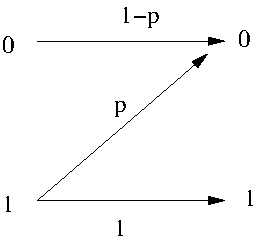
\includegraphics[scale=0.5]{capacidad/zchannel}
  \end{center}
  \caption{Diagrama: Z-channel}
  \label{fig:Gal}
\end{figure}

Para un Z-channel, la distribucion de probabilidades de I(X;Y) es diferente, por lo que obtenemos un máximo diferente:

$$ C_{Z} = 1 - \left(\frac{1}{2}*H(p)\right) $$ \cite{tallini}

Por lo tanto,

$$ C_{Z} = \log_2\left(1+(1-p) p^{p/(1-p)}\right) $$


\begin{figure}[th]
  \begin{center}
    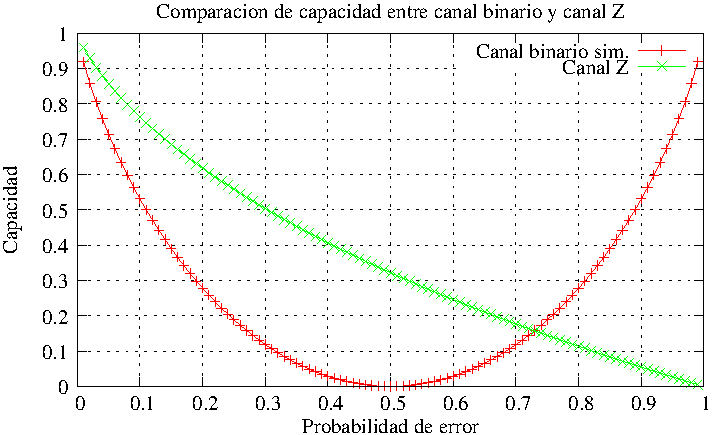
\includegraphics[scale=0.9]{capacidad/comparacionBZ}
  \end{center}
  \caption{Diagrama: Azul: Capacidad de canal binario Verde: Capacidad de canal Z}
  \label{fig:CompBZ}
\end{figure}


\subsection{Filtros de bloom}
Como se discutió en la seccion [TODO], la colisiones de símbolos son inherentes a la modulación seleccionada.
En la modulacion OOK utilizada en un medio óptico, solo los ‘1’s transmitidos pueden interferir con ‘0’s.
Este comportamiento puede ser modelado como un canal-Z porque la superposición de pulsos de luz individuales representando ‘1’s puede solamente ser identificados como un ‘1’s, por que la interferencia solamente puede ser aditiva. De esto se desprende que un ‘0’ recibido es un signo inequívoco de la ausencia de pulsos en el slot de tiempo leido.
Una buena estructura para representar este tipo de datos es el filtro de Bloom [TODO], que se utiliza generalmente en técnicas de hashing, utilizándolo para tests muy rápidos (O=1) de pertenencia de un miembro en un set.
La manera en que se implementó este algoritmo en el sistema propuesto se basa es copiar cada bit en K slots del frame transmitido, siendo el frame la representación física del filtro de Bloom. 
En el extremo receptor es suficiente para recibir un solo ‘0’ entre las K copias del bit, para correctamente inferir que el bit original era originalmente un ‘0’, mientras que si el bit original era un ‘1’, las colisiones no tienen efecto debido a la naturaleza del canal-Z.

%As discussed in section 2, this leads to collisions. Since the modulation format is OOK, only transmitted ‘1’s can interfere with ‘0’s.
%This behaviour can be modelled as a Z-channel because the superposition of individual light pulses representing ‘1’s
%can only be identified as a ‘1’, but a received ‘0’ is an unmistakable sign of the absence of pulses in a given time slot.
%We found that the Bloom filter [2] provides a convenient structure to correct for errors in this type of channel. This
%technique is borrowed from hashing algorithms and is used to test whether an element is member of a given set. The
%way that we implement this algorithm relies on copying every bit in K slots of the transmitted frame. On the receiving
%end it is sufficient to receive a single ‘0’ out of K copies in order to correctly retrieve the original transmitted ‘0’,
%whereas collisions have no effect on ‘1’s.

\section{Espectro ensanchado}

Repetido en \ref{espectroensanchado} ??
\subsection{Time-hopping con filtros de bloom}

\section{Minimización de peso de Hamming}
%% extraido de dline-pub.text

Repasando, el esquema propuesto basado en time-hopping CDMA se basa en la interferencia entre símbolos para obtener confidencialidad, ya que los datos de los otros usuarios actuan efectívamente como ruido.
La interferencia inter-símbolo, como fue discutida en la seccion \ref{principle}, causa errores que debe ser corregidos. Como dichos errores reducen el ancho de banda utilizable del canal, es deseable reducir la interferencia hasta un punto donde se maximize, sin comprometer la seguridad del sistema. Para reducir la interferencia, no es aconsejable modificar o introducir patrones en el generador criptograficamente seguro de numeros aleatorios, ya que comprometeria la seguridad de todo el sistema al introducir predictabilidad en las posiciones de los símbolos (Ej. usando códigos ortogonales como en Ref.~\cite{Nadarajah2006}.), efectivamente dejando de ser criptograficamente seguro.
En lugar de esto, se adopto una estrategia que aprovecha el echo que un sistema óptico puede ser modelado como un canal-Z.

%This channel presents a Shannon limit of $ C_{Z} = \log_2\left(1+(1-p) p^{p/(1-p)}\right),$ where $p$ is the probability of error~\cite{Tallini:02}.

Esta propuesta, y aqui esta el nucleo de la invencion propuesta en esta tesis, es la de aprovechar la naturaleza asimetrica del este tipo de canal, en donde solamente el símbolo ``1'' causa interferencia, ya que los ``0'' no se interfieren. \footnote{Aunque en un sistema óptico real, existe efectivamente una pequeña diferencia ya que un ``0'' nunca es representado con una potencia de laser de cero watts.}
En otras palabras, la interferencia de un canal-Z es proporcional al peso de hamming del símbolo transmitido.
El peso de Hamming de un símbolo es simplemente la cantidad de bits en ``1'' del mismo. El algoritmo de Minimización de peso de Hamming consiste en una codificación en donde cada símbolo binario es convertido en un equivalente de mayor longitud, tieniendo solamente una mínima cantidad de dígitos en ``1''. Aplicando esta codificación que minimiza el peso de Hamming y transmitiendo el símbolo resultante, se obtiene una menor interferencia en un canal Z.
Intuitivamente, expandir el símbolo original a uno de mayor longitud decrementaria el ancho de banda del canal; pero como las simulaciones numéricas muestran (ver sección \ref{simulations}) a medida que la interferencia inter-símbolo se reduce, el ancho de banda adicional utilizado por los algoritmos de FEC tambien se reducen, compensando por el incremento del largo del símbolo y logrando un mayor ancho de banda neto del sistema.
Podemos decir que un número binario normal de largo L posee un peso variable de Hamming, con L/2 siendo el promedio, cero siendo el mínimo y L siendo el máximo peso de Hamming.
La técnica de reduccion de peso de Hamming (HW) da buenos resultados reduciendo a HW=2, logrando un buen balance entre la reducción de interferencia y el largo de símbolo.
Adicionalmente, es deseable en un sistema de seguridad que no se revele ninguna información acerca de los símbolos transmitidos. Por ejemplo si transmitieramos el número cero, representado por todos sus dígitos en cero, seria trivial identificarlo sin importar si se aplica cualquier tipo de time-hopping. Para evitar estos ataques que utilizan estadísticas acerca del peso de hamming, la codificación exige que el peso de hamming sea fijo en todos los símbolos. Esto causa una ligera perdida en el ancho de banda pero hace imposible inferir cualquier tipo de información acerca del símbolo transmitido analizando estadisticas de tráfico de los datos transmitidos.

\begin{table}[t]
\begin{center}
\begin{tabular}{c c c}
Datos & entrada HW= 0 to 3 & Expandida HW=2\\
\hline\hline
0 & 000 & 00011\\
1 & 001 & 00110\\
2 & 010 & 00101\\
3 & 011 & 01100\\
4 & 100 & 01010\\
5 & 101 & 01001\\
6 & 110 & 10001\\
7 & 111 & 10010\\
\end{tabular}
\caption{Tambla de minimización de Hamming para símbolos de 3-bits}
\label{hwtable}
\end{center}
 \end{table}
 
\section{Expansión de símbolo}
La minimización del peso de hamming conlleva una necesaria conversión del símbolo original a otro que necesariamente tendra mayor longitud, o sea, una expansión del símbolo.
Esta operación puede realizarse de muchas maneras, pero un algoritmo muy eficiente es utilizar una tabla de lookup (ver tabla~\ref{hwtable}), donde un símbolo de largo L es utilizado como el índice en la tabla, y el resultado es el símbolo expandido, que tiene un largo N\textgreater L.
Por motivos prácticos y de optimización, es deseable que L sea 8 u 16 bits, por lo que la tabla contendrá 256 o 65536 entradas respectivamente.
Al aplicar la minimización de peso de hamming a símbolos de 8 o 16 bits de longitud, son necesarios 256 o 65536 símbolos de salida con un HW=2. En el caso de símbolos de entrada de 8 bits, la longitud del símbolo de salida sera de 363 bits, mientras que para 8 bits de entrada, el simbolo expandido con HW=2 tendra 24 bits de longitud.
Puede observarse que el número de símbolos únicos con HW=2 y N=363 no es exáctamente 65536 sino 65703, esto significa que existen muchas tablas de expansión.
La tabla seleccionada y el orden de la misma no son importantes para el resultado final, observando la condición que dos nodos comunicandose deberan utilizar idénticas tablas.
%In general more bits transmitted per frame the more efficient the protocol will be. \textbf{PORQUE IN GENERAL? CUANDO FALLA?} 


\section{Sistema completo}
%% De orte.tex
El sistema propuesto esta compuesto primeramente de una capa de acceso, donde es implementada la codificación CDMA y corrección de errores, y una capa física basada o bien en una red óptica con similaridades a redes PON, o una red sónica de broadcast.
La capa de acceso es implementada utilizando CDMA del tipo time-hopping, donde cada uno de los $128$ ONUs posibles codifica su información en bits y los envia en un slot seleccionado de manera aleatoria en un frame de $356$ slots\footnote{ Estos valores pueden por supuesto variar de acuerdo a los parametros como error aceptable y cantidad de clientes máxima.}. De esta manera, ocurriran multiples colisiones entre diferentes ONUs pero seran subsanadas por la capa de corrección de errores que garantiza una transmisión de datos virtualmente\footnote{aunque es implosible eliminar totalmente los errores, un BER de 10E-12 se considera libre de errores} libre de errores.

Nota rque la sincronizacion es realizada solo a nivel de bit-slot, en contraste con técnicas como TDMA que deben sincronizar a nivel de frame. También se elimina el requerimiento de una transmisión ordenada en el tiempo; en el esquema propuesto ambos clientes comunicantes pueden empezar su comunicación en cualquier momento, de manera similar al comportamiento del protocolo ethernet.
Un cierto ONU $X$ puede recibir mensajes de otro ONU $Y$ si y solo si $X$ posee la {\em clave} de $Y$, y vice versa. De esta manera, si un cierto grupo de ONUs desean comunicarse sobre VLAN, es requerido que cada una en el grupo conozca todas las otras {\em claves}.

Los flujos de datos de las ONU's se codifican con las siguientes técnicas de corrección de errores (Fig. \ref{arch:chain}):

Reed-Solomon ($223/255$) y algoritmos LDPC ($1024\times512$ matrix) (ver \cite{Moon:05} y sus referencias), ademas de un filtro de Bloom con $K=4$~\cite{Bloom70space/timetrade-offs}.

La seleccion de estos algoritmos de corrección de errores fue influenciada al considerar al canal de comunicaciones como el denominado canal Z, que posee un limite de Shannon de $ C_{Z} = \log_2\left(1+(1-p) p^{p/(1-p)}\right),$ donde $p$ es la posibilidad de recibir un error al transmitir un bit.
Este limite de capacidad es mayor que el límite en una canal simétrico sin memoria \cite{Tallini:02}.

\section{Aplicación en distintos medios físicos}
\subsection{Redes ópticas}
% de orte.text
\begin{figure}[!t]
  \centering
    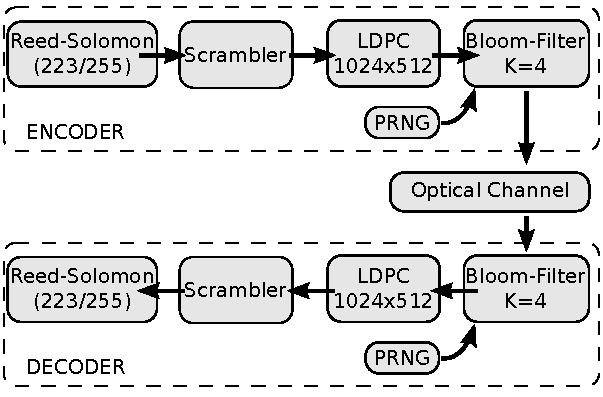
\includegraphics[width=3in]{orte01.pdf}
    \caption{Proposed network design: Access Layer}
    \label{arch:chain}
\end{figure}
% Fiber		Es grave el efecto de la dispersion?  Sugerimos dispersion shifted G.653? O son muy caras?
% splitter	No 1x128 commercially available (attenuation $\leq 27\,dB$)
% DFB		http://cess-dk.com/gfx/upload/PX2-1541SF.pdf ( min $\simeq-1\,dB$)
% APD		http://pdf.dzsc.net.cn/200810212/286762.pdf ( max $\simeq-27\,dB$)
% EDFA		http://www.lambdaphoto.co.uk/pdfs/EDFADatasheet.pdf

Al adaptar el sistema propuesto a una red óptica, la topología de misma debe ser de tipo estrella (ver Fig.\ref{arch:fig1}) donde splitters ópticos redistribuyen el tráfico proveniente de cada ONY a todo el resto permitiendo comunicaciones punto-a-punto asi como punto-a-multipunto entre hasta $128$ ONUs.
%Traffic redistribution is made by optical splitters at the redistribution hub that introduces high attenuation to optical streams.
Un amplificador óptico de fibra de Erbio (Erbium-Doped Fiber Amplifier, EDFA) localizado entre los splitters en el repetidor óptico incrementa la potencia óptica para contrarrestar las perdidas en la red. 

La modulación utilizada para las señales ópticas es RZ \footnote{La modulacíon RZ o ``Return to Zero'' es la mas común utilizada en fibras ópticas, aunque por razones técnicas en ralidad el laser nunca retorna a cero. Esto tiene consecuencias para el sistema propuesto como se vera mas adelante.} con velocidades previstas de hasta $10$~Gbps por un laser DBF de $2$~dBm de potencia y $1550$~nm de color/frecuencia. Estos parametros permiten una transmisión de hasta $10$~km entre los nodos si se utiliza fibra óptica mono-modo estandard (ITU-T G.652) hacia el repetidor óptico.

En este hub, un spliter de $128\times 1$ maneja el tráfico de todos los ONUs y es luego redistribuido por el correspondiente splitter de $1\times 128$, canalizando el trafico mezclado de cada ONU a travéz de la fibra de bajada, paralela a la fibra de subida.
La atenuacion de los splitters centrales ($\simeq25$~dB cada uno) sumado a la atenuación propia de la fibra óptica y perdidas por inserción ($\simeq2$~dB y $\simeq1$~dB por tramo) contribuyen a las altas pérdidas que este sistema debe compensar ($\simeq28$~dB en ambos canales de subida y bajada).

De utilizarse sin ningun tipo de amplificación, la atenuación que una señal sufriria entre dos ONUs es la suma de la atenuación de ambos tramos, o sea $\simeq56$~dB, que es un valor extremadamente alto fuera del alcance de la tecnología de detección disponible al momento de la escritura de esta tesis.

Sin embargo es posible pasar por etapas de amplificación intermedias para obtener niveles de señal adecuados. Para proveer la amplificación requerida, un EDFA con $\geq27$~dB de ganancia es colocado entre ambos splitters. Este EDFA incrementa la potencia del tráfico a la salida del primer splitter, elevando la potencia de cada '1' de $\simeq-26$~dBm a $1$~dBm a la entrada del segundo splitter, que sera reducida nuevamente por el mismo a un nivel de potencia de $-27$~dBm, que esta dentro de los parametros aceptables de un fotodetector (PD) comercial de alta sensibilidad (Aprox. ($-28$~dBm)).

La potencia máxima de salida del PD no es un parámetro crítico ya que simulaciones [CUALES?] muestran que solamente se produciran colisiones de hasta diez `1' en un slot, y esto con una posibilidad extremadamente baja.

Aún considerando una ganacia de EDFA constante, la potencia de entrada óptica del PD seria menor ($-17$~dBm) que la que son capaces de soportar dispositivos comerciales ($\sim -5$~dBm).
El nivel de bit `0' es dado por la adición de todos los bits `0' transmitidos por todas las $128$~ONUs.
El nivel de decisión del receptor deberia ser capaz de separar entre este estado y aquel de un simple ONU transmitiendo un solo bit en `1'.
De esto se desprende que la potencia de transmisión del bit `0' debe ser la menor posible, o lo que es lo mismo, el radio de extinción del laser DBF debe ser alto.
El radio de extinción (`1'$/$`0' radio de potencia pico) mínimo requerido por el sistema se discute en las simulaciones numéricas a continuación:

% As collisions occur in this scheme minimal powers are such for the case of a single active Tx in a bit slot. In a bit slot with collisions (two or more `1' bits) power increase could be a concern to APD operation
% Optical transmission is performed by a $2$~dBm $1550$ nm DFB-laser generating a
% $10$ Gb/s RZ modulated optical signal, that is transported by up to $10$
% km upstream fiber (ITU-T G.652) to a redistribution hub (see
% Fig.~\ref{arch:fig1}).
\begin{figure}[!t]
  \centering
    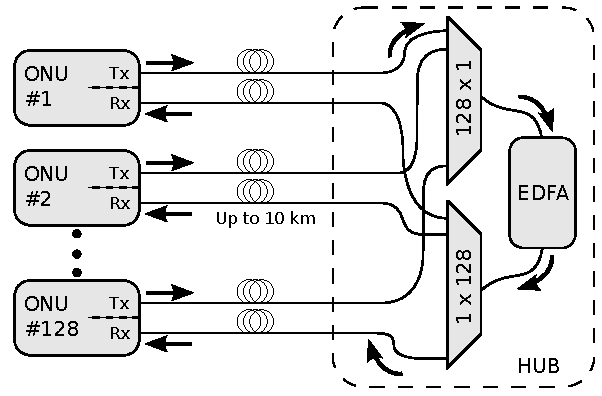
\includegraphics[width=3in]{orte02.pdf}
    \caption{Diseño de red propuesto: Capa óptica}
    \label{arch:fig1}
\end{figure}
% Upstream traffic from all ONUs are merged by a $128\times 1$ splitter and then again redistributed by another splitter $1\times 128$ that channels back merged traffic to each ONU through a downstream fiber identical and parallel to the upstream one.
% Splitters' attenuation ($\simeq25$~dB, estimated) contribute, as well as fiber attenuation and insertion losses ($\simeq2$~dB and $\simeq1$~dB per stretch), amount to high total attenuation ($\simeq28$~dB at each upstream and downstream paths).
% In order to make the system workable it is proposed to place a single EDFA optical amplifier ($\geq27$~dB gain) between both splitters.
% This EDFA rises merged traffic power at first splitter output ($\simeq-26$~dBm `1' active Tx) delivering enough power ($1$~dBm, `1' active Tx) at second splitter input to assure power reaching each ONU ($-27$~dBm, `1' active Tx) allows proper reception by a high sensitivity APD ($-28$~dBm).

\subsection{Redes acústicas}
% de newJIS_140512-1.pdf (paper JIS)
\begin{figure}[!t]
  \centering
    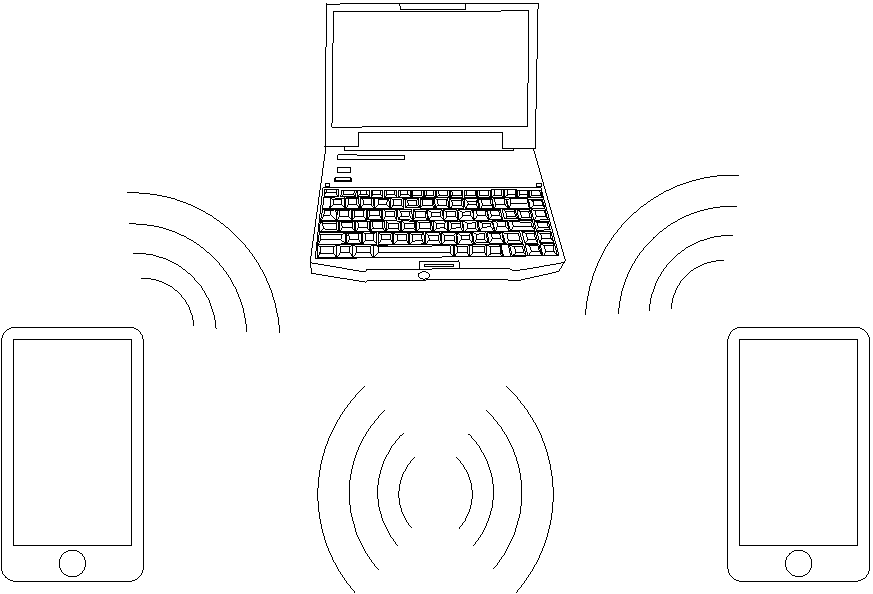
\includegraphics[width=3in]{compucelus.pdf}
    \caption{El diseño de red acústica propuesta puede contener nodos heterogeneos, tales como celulares móviles o computadoras personales.}
    \label{arch:chain}
\end{figure}

Como se discutió anteriormente [DONDE?] es posible utilizar como capa física cualquier canal de comunicaciónes cuyo modelo de ruido o probabilidad de error sea aproximado al de un canal-Z. Un canal óptico es un ejemplo, pero es posible realizar un canal-Z con redes acústicas si se utilizan ciertas modulaciónes y párametros.

Los enlaces ópticos presentan como mayor desventaja la necesidad de, o bien una fibra óptica entre los nodos comunicantes, o que exista visibilidad directa entre ambos nodos, una condición que no puede ser garantizada en muchos ambientes de trabajo. Ademas, los sensores ópticos requeridos generalmente no estan presentes en los clientes y deben ser instalados separadamente.

Sin embargo utilizar un canal acústico tiene como ventaja poder utilizar hardware pre-existente en la mayoria de los potenciales clientes, como parlantes o micrófonos estandard, elementos muy comunes en dispositivos de información actuales [6]. Además, no es necesaria la visibilidad directa mientras ambos nodos esten localizados a pocos cm o metros de distancia, con bajo nivel de volumen.

Pero en contraste con otras tecnologías como RF o enlaces ópticos, la naturaleza del canal de sonido y la facilidad para interceptar o registrar comunicaciones utilizando este medio hace necesaria que la privacidad sea un requerimiento esencial. Muchos sistemas de comunicacion de audio han sido propuestos [7], pero hasta donde fue posible investigar, el problema de la privacidad en este tipo de comunicaciones ha sido solucionada solamente en la capa de aplicación, o sea en alto nivel. Este trabajo presenta una aproximación a la seguridad y privacidad desde la capa física, basada tambien en time-hopping CDMA, similar a aquella presentada en las referencias [8, 9]. En este trabajo se presenta una red segura acústica punto-a-punto y punto-a-multipunto de corto rango y bajo consumo, que no requiere de ningun hardware adicional en clientes moviles.
Establecer un enlace privado entre dispositivos moviles previamente desconectados requiere cierto nivel de interacción por parte del usuario que es usualmente ignorado [5]. Sin embargo, cuando la privacidad se brinda desde la capa física, la intervención del usuario es minimizada. Este es el caso de esta propuesta.

Un escenario válido para la aplicación de esta tecnología podria ser la validación de transacciones financieras pequeñas tales como terminales PoS (Point of Sale) o cajeros automaticos (ATM) utilizando un dispositivo movil (Ej. un smartphone) sin modificaciónes de hardware. Una tecnología similar que se utiliza en estos casos es la denominada Near Field Communications (NFC) [10], un protocolo inalámbrico que requiere hardware especializado que al momento de escritura de esta tesis no se encuentra disponible en la mayoria de los dispositivos moviles.

\subsection{Redes acusticas: Arquitectura}

Una ventaja muy importante del sistema acústico propuesto es su simplicidad, requiriendo solamente un emisor de sonido (parlante), un receptor (micrófono) y un canal de transmisión de sonido que puede ser aire (y en casos mas especializados, agua). Ambos requerimientos estan generalmente disponibles en computadoras, notebooks, tablets y telefonos celulares modernos. 
El esquema lógico es el mismo que el descrito anteriormente: Time-hopping CDMA seguro, códigos correctores de erroes y un método de sincronización a nivel de bit.
Como resultado, el sistema provee canales unidireccionales a los usuarios que sirven tanto para comunicaciones punto-a-punto como punto-a-multipunto. Comunicaciones bi-direccionales pueden establecerse utilizando dos canales separados (Ej. utilizando dos codigos CDMA diferentes), o empleando el mismo canal de manera half-duplex, aunque este último modo de funcionamiento necesita de desarrollo adicional y no es el objetivo de esta tesis.
En las próximas secciones se describe el sistem en mayor detalle.

